%%% File encoding: UTF-8
%% äöüÄÖÜß  <-- no German Umlauts here? Use an UTF-8 compatible editor!

%%% Magic comments for setting the correct parameters in compatible IDEs
% !TeX encoding = utf8
% !TeX program = pdflatex 
% !TeX spellcheck = en_US
% !BIB program = biber

\documentclass[master,english]{hgbthesis}
% Permissible options in [..]: 
%   Type of work: diploma, master (default), bachelor, internship 
%   Main language: german, english (default)
%%%----------------------------------------------------------

\RequirePackage[utf8]{inputenc}		% Remove when using lualatex or xelatex entfernen!
\usepackage{graphicx}
\usepackage{svg}
\usepackage{minted}
\usepackage{listings}

% -----------------------------------------------------
\newenvironment{code}{\captionsetup{type=listing}}{}
% -----------------------------------------------------
% -----------------------------------------------------
\newcommand{\mysubsubsection}[1]{{\subsubsection{\textbf{#1}}}}
\newcommand{\mentionedtext}[1]{{\textit{{#1}}}}
\newcommand{\sourceDir}{./sources}
\newmintedfile[yamlFile]{yaml}{
	linenos=true, 
	frame=single, 
	breaklines=true, 
	tabsize=2,
	numbersep=5pt,
	xleftmargin=10pt,
	baselinestretch=1,
	fontsize=\footnotesize
}
% -----------------------------------------------------
\graphicspath{{images/}}    % location of images and graphics
\logofile{logo}				% logo file = images/logo.pdf (use \logofile{} for no logo)
\bibliography{references.bib}  	% name of bibliography file (references.bib)

%%%----------------------------------------------------------
% Title page entries
%%%----------------------------------------------------------

%%% Entries for ALL types of work: --------------------------
\title{Implementation of an Enterprise Service Bus with OpenShift and Camel}
\author{Ing. Thomas Herzog B.Sc}
\programname{Software Engineering}
\placeofstudy{Hagenberg}
\dateofsubmission{2018}{06}{01}	% {YYYY}{MM}{DD}

%%% Entries for Bachelor theses only: -----------------------
%\thesisnumber{XXXXXXXXXX-A}   %e.g. 1310238045-A  
% (Stud-ID, A = 1st Bachelor thesis)
%\semester{Fall Semester 2017} 	% Fall/Spring Semester YYYY
%\coursetitle{Introduction to Trivial Problems 1} 
\advisor{DI (FH) Peter Kulczycki}

%%% Restricted publication license instead of CC (master only):
\strictlicense

%%%----------------------------------------------------------
\begin{document}
%%%----------------------------------------------------------

%%%----------------------------------------------------------
\frontmatter							% title part (roman page numbers)
%%%----------------------------------------------------------

\maketitle
\tableofcontents

\chapter{Preface}






 	% preface is optional
\chapter{Abstract}
An Enterprise Service Bus (ESB) is a crucial part of an enterprise, which connects the enterprise to its partners, customers, and other branches. The appearance of containerization, cloud services, and the microservice architecture have provided new possibilities for implementing and running an ESB. But, an ESB is commonly used by large conservative enterprises, which don't adapt new technologies fast, and wait until a new technology has proven itself. Especially the cloud is something the industry denied to use for a long time, because of the fact, that the infrastructure and data are managed and maintained by external service providers. \\ 

These days, we live in the so called cloud age, whereby global enterprises like Red Hat or Amazon provide cloud services such as Platform as a Service (PaaS), which can scale with the business. Enterprises start to consider to move their ESB installations to the cloud to profit from the cloud service provided features. Moving an ESB to the cloud will be a long term process for an enterprise, because the established processes for development, running, and managing the ESB will have to change. \\

This thesis has the goal to give the reader an overview of the cloud related concepts and technologies such as, Infrastructure as Code (IaC) and Docker, which are the base for cloud services. The implemented ESB prototype,  is  available at \url{https://github.com/cchet-thesis-msc/prototype}, and shows how an ESB could be implemented on a PaaS platform. \\




%%%----------------------------------------------------------
\mainmatter          			% main part (arabic page numbers)
%%%----------------------------------------------------------

\chapter{Introduction}
\label{cha:intro}

\section{Motivation}
\label{sec:intro-motivation}
Large enterprises work with several independent applications, whereby each application covers an aspect of their business. In general, these applications are from different vendors, implemented in different programming languages, and with their own life-cycle management. To provide a business value to the enterprise, these applications are connected via a network, and they contribute to a business workflow. The applications have to exchange data, which is commonly represented in different formats and versions. This leads to a highly heterogeneous network of applications, which is hard to maintain. \\

The major challenge of an IT department is the integration of independent applications into the enterprise application environment. The concept of Enterprise Application Integration (EAI) provides patterns, which help to define a process for the integration of applications into a heterogeneous enterprise application environment. One of these patterns is the Enterprise Service Bus (ESB), which is widely used in the industry\cite{EIP}. \\

Often, the term ESB application is used to refer to an ESB, which integrates internal and external hosted applications. But an ESB is a software architectural model, rather than an application. The term could have been established by the usage of middleware such as JBoss Fuse, which provides tooling to integrate applications into an ESB. Red Hat JBoss Fuse is be based on the JBoss Enterprise-Application-Platform (JBoss EAP), where all integration services run in the same runtime environment\cite{Fuse2018}. \\

With the appearance of cloud solutions, such as Platform as a Service (PaaS), it is now possible to move an ESB from a dedicated environment to a cloud environment, whereby each integration service runs in its own runtime environment, rather than joining an existing runtime environment. The concept of Integration Platform as a Service (IPaaS) is built on top of PaaS, and enhances a common PaaS solution with the integration features required by EAI\cite{PaaS2015, iPaaSP12015}. \\

Thus, enterprises can reduce the effort in implementing and maintaining an ESB, integrating applications into the ESB, and reducing the costs of an ESB, by using a consumption based pricing model. The cost are reduced due to the fact, that the ESB can scale down when its load decreases, whereby less resources are consumed, which have to be paid for.

\section{Objectives}
\label{sec:intro-objectives}
This thesis aims to implement an ESB on Openshift PaaS. An ESB is different to a Service Hub, because the ESB is a distributed system by design, whereby for instance, transformation is not centralized, as it is with an Service Hub. A Service Hub has a central component, which performs transformation, routing and orchestration, whereby the scaling is limited by the hardware capabilities of the central hub. Additionally, the hub component of a Service Hub represents a single point of failure\cite{EIP}. \\

Commonly, an ESB is implemented with the help of middleware such as JBoss Fuse, which is based on the JBoss EAP. The concepts of PaaS and IPaaS are in general new to the industry, which commonly hosts their integration services in their own data centers, due to the lack of trust for cloud solutions and knowledge about the new approaches such as the microservice architecture\cite{Openshift2018}. \\

Before implementing an ESB, which runs on a PaaS platform such as Openshift, it is necessary to understand the new concepts such as Infrastructure as Code (IaC) or containerization with Docker, which are covered in the following chapters. The microservice architecture and cloud services such as PaaS are becoming more important for the software industry, because of the features they provide. For instance, Red Hat is currently moving its ESB middleware JBoss Fuse to the cloud, whereby JBoss Fuse will fully rely on Openshift, and the integration services will have to be implemented as microservices. This has a huge impact on Red Hats customers, who are used to JBoss Fuse on top of JBoss EAP. \\

This thesis was commissioned by the company Gepardec IT Services GmbH, a company, which is working in the area of Java Enterprise and Cloud Development. The migration from a monolithic ESB to a microservice structured ESB, which is hosted in a PaaS environment, is a major concern for them. The migration from a monolithic ESB to a microservice structured ESB will be a major challenge for their customers, because microservice architecture and cloud solutions are mostly new to them.  \\

Over the past years a huge technology dept has been produced by the industry, due to the monolithic architecture of their applications and little refactoring work on their application sources. It will be hard for them to reduce the accumulated technology dept, which they will have to, to keep competitive. Gepardec sees a lot of potential for their business and their customers in this new approach of implementing and hosting an ESB. \\

The term \quotes{monolithic ESB} refers to an ESB implementation, whereby all integration services are part of a single application, and therefore, are part of the application life-cycle, instead of having an own life-cycle per integration service. An integration service is a service, which integrates two or more other service with each other, by handling aspects like data transformation, routing, or security, between the integrated services.  
\chapter{Infrastructure as Code}
\label{cha:iac}
Infrastructure as Code (IaC) is a concept to automate system creation and change management with techniques from software development. Systems are defined in a Domain Specific Language (DSL), which gets interpreted by a tool, which creates an instance of the system or applies changes to it. IaC defines predefined, repeatable routines for managing systems \cite{Morris2016}. IaC descriptions are called templates, cookbooks, recipes or playbooks, depending on the tool. In the further course, the IaC definitions will be called templates. The DSL allows to define resources of a system such as network, storage and routing descriptively in a template. The DSL abstracts the developer from system specific settings and provides a way to define the system with as little configuration as possible. The term system is used as a general description. In the context of IaC, a system can be anything which can be described via a DSL.

\section{The Need for Infrastructure as Code}
\label{sec:iac-need}
In the so called iron age, the IT systems were bound the physical hardware and the setup of such a system and its change management were a long term, complex and error prone process. These days, we call such systems legacy systems. In the cloud age, the IT systems are decoupled from the physical hardware and in the case of PaaS they are even decoupled from the operating system \cite{Morris2016}. The IT systems are decoupled from the physical hardware and operating system, due to the fact, that cloud providers cannot allow their customer to tamper with the underlying system and hardware. In general, the hardware resources provided by a cloud provider are shared by multiple customers. \\

With IaC it is possible to work with so called Dynamic Infrastructure Platforms, which provide computing resources, where the developers are completely abstracted from the underlying system. Dynamic infrastructure platforms have the characteristic to be programmable, are available on-demand and provide self service mechanisms, therefore we need IaC to work with such infrastructures \cite{Morris2016}. Systems deployed on a dynamic infrastructure platform are flexible, consistent, automated and reproducible. \\

Enterprises which stuck to legacy systems face the problem that technology nimble competitors can work with their infrastructures more efficiently, and therefore can demand lower prices from their customers. This is due to the IaC principles discussed in Section \vref{sec:iac-principles}. Over a short period of time, enterprises will have to move to IaC and away from their legacy systems to stay competitive. The transition process could be challenging for an enterprise, because they lose control over the physical hardware and maybe also over the operating system. Maintaining legacy systems has the effect that someone is close to the system and almost everything is done manually. IaC has the goal to automate almost everything, which requires trust for the cloud providers, who provide the computing resources and the tooling, which provides the automation. A well known problem, which enterprise will face, is the so called Automation Fear Spiral, which is shown in Figure \vref{fig:automation-fear-spiral}.

\begin{figure}[htbp]
	\centering
	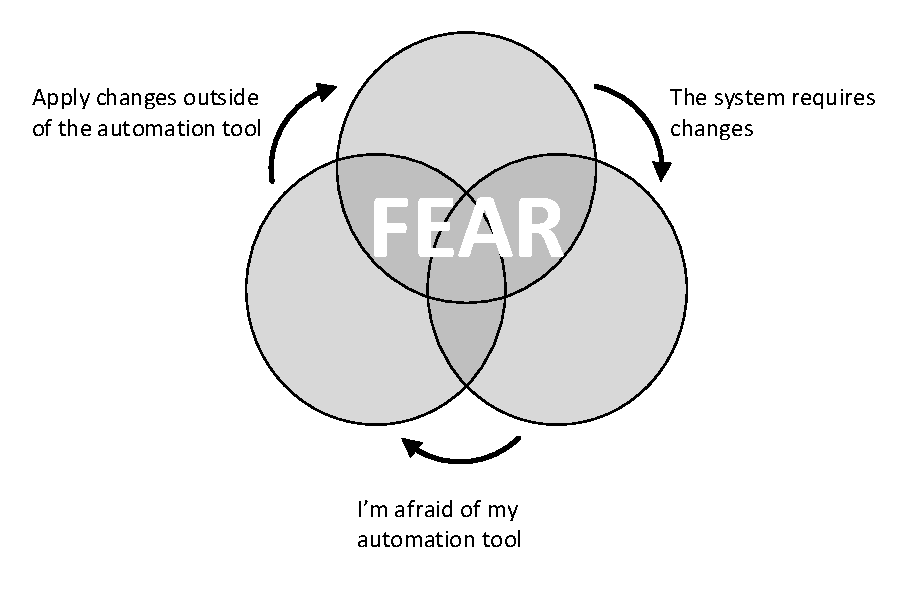
\includegraphics[scale=1]{images/automation-fear-spiral.pdf}
	\caption{Automation Fear Spiral}
	\label{fig:automation-fear-spiral}
\end{figure} 

Because of no trust for the automation, changes are applied manually to the systems and outside the defined automation process. If the system is reproduced, definitions may be missing in the templates, which leads to an inconsistent system. Therefore, enterprises have to break this spiral to fully profit from IaC \cite{Morris2016}. \\

When enterprises have moved their legacy systems to IaC, they can not only manage their systems faster, they also can profit from the principles of IaC as discussed in Section \vref{sec:iac-principles}. With IaC, systems are less complicated to manage, changes can be applied without fear, and the systems can easily be moved between environments. This provides the enterprises with more space to maneuver, systems can become more complex but still easy to manage, the systems can be defined and created faster which could lower costs.    

\section{Principles of Infrastructure as Code}
\label{sec:iac-principles}
The principles of IaC solve the problems of systems of the iron age. In the iron age the creation and maintenance of systems were a long, complicated and error prone process which consumed a lot of resources and time. With the decoupling of the physical hardware from the system, the creation and maintenance of the system has become simple, due to the IaC DSL and tooling. 

\subsection{Infrastructures are Reproducible}
\label{sec:iac-principles-reproducibility}
With IaC, systems are easy reproducible. It is possible to reproduce the whole infrastructure or parts of it effortlessly. Effortless means, that no tweaks have to be made to the templates or during the reproduction process and there is no need for a long term decision process about what has to be reproduced and how to reproduce it. To be able to reproduce system effortlessly is powerful, because it can be done automatically, consistently and with less risk of failures \cite{Morris2016}. The reproducibility of a system is based on reusable templates which provide the possibility to define parameters, which are set for the different environments as shown in Figure \ref{fig:reproduce-infrastructure}.

\begin{figure}[htbp]
	\centering
	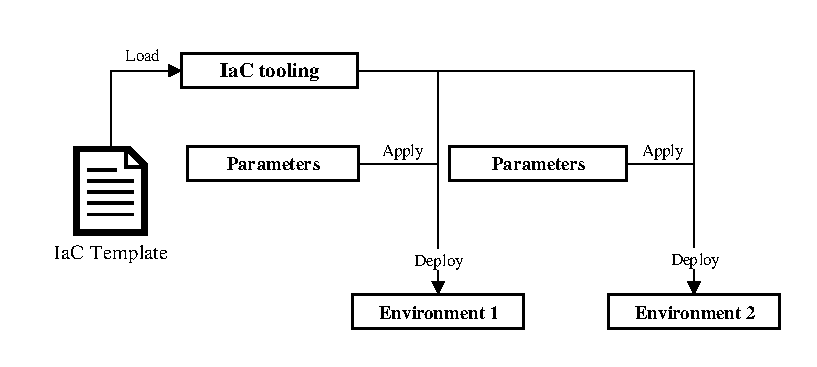
\includegraphics[scale=0.95]{images/reproduce-infrastructure.pdf}
	\caption{Schema of a parametrized infrastructure deployment}
	\label{fig:reproduce-infrastructure}
\end{figure} 

\subsection{Infrastructures are Disposable}
\label{sec:iac-principles-disposable}
Another benefit of IaC is that systems are disposable. Disposable means, that systems can be easily destroyed and recreated. Changes made to the templates of a system does not have to be applied on an existing system, but can be applied by destroying and recreating the system. An requirement for a disposable system is, that it is understood that systems will always change. Other systems relying on a disposable system need to address that the system could change at any time. Systems must not fail because a disposable system disappears and reappears again because of an redeployment \cite{Morris2016}.

\subsection{Infrastructures are Consistent}
\label{sec:iac-principles-consistency}
Systems managed with IaC are consistent, because they are defined via a template and all instances are an instance of the template, with the little configuration differences defined by parameters. As long as the system changes are managed by IaC, the system will stay consistent, and the automation process can be trusted. \\

In Listing \vref{src:iac-template-docker-compose} an example for an IaC template is shown, which defines a Docker Compose service infrastructure for hosting a Wildfly server instance \cite{Wildfly2017, DockerCompose2018}. This system can consistently be reproduced on any environment supporting Docker, Docker Compose and providing values for the defined parameters. \\

\begin{code}
	\yamlFile{\sourceDir/iac-docker-compose.yml}
	\caption{Example for an IaC template for Docker Compose}
	\label{src:iac-template-docker-compose}
\end{code}

\subsection{Actions are Repeatable}
\label{sec:iac-principles-repeatability}
Building reproducible systems, means that any action applied to the system should be repeatable. Without repeatability, the automation cannot be trusted and systems wouldn't be reproducible. An instance of a system in another environment should be equal to any other system instance, except for the configurations defined by parameters. If this is not the case, then a system is not reproducible, because it will have become inconsistent \cite{Morris2016}. \\

IaC is a concept which makes it very easy to deal with systems in the cloud age. Enterprises can make use of IaC to move their legacy systems to the cloud, where they can profit from the principles of IaC. Nevertheless, before an enterprise can profit from IaC, it has to apply clear structures to their development process, as well as sticking to the principles of consistency and repeatability. For experienced administrators, who are used to maintain systems manually, it could sometimes be hard to understand why they are not supposed to perform any actions on the system manually anymore, nevertheless that a manual change could be performed faster. Being capable to reproduce a system at any time with no effort,  or applying changes on an existing system in a predefined and consistent manner,  makes enterprises very flexible and fast. Enterprises will not have to fear future changes in requirements and technologies of their systems anymore.    




\chapter{Containerization with Docker}
\label{cha:containerization-docker}
Docker is a tool for creating, provisioning and interacting with Linux Containers (LXC) \cite{Docker2018,LXC2018}. LXC are a lightweight version of virtualization, which does not have the resource impact of a full virtualization such as Operating System (OS) virtualization. The differences of LXC and a Virtual Machine (VM) are covered in Section \ref{sec:docker-virtualization-vs-containerization}. Docker has become very popular over the past years, due to the fact, that it made it possible to easily work with LXC. Docker relies strongly on the principles of IaC which has been discussed in Chapter \ref{cha:iac}. When using Docker, Linux Containers are often referred to as Docker Containers. \\

Containerization is a key factor when hosting applications in the cloud, because the applications are normally packaged in images and run as containers on the cloud platform. Containerization provides features for a fast, effortless and consistent way of running applications in the cloud, which is discussed in the following Section \ref{sec:docker-need-for-containerization}.

\section{The need for Containerization}
\label{sec:docker-need-for-containerization}
Containerization is a key factor for cloud platforms such as PaaS, where each application runs in its own isolated environment, called a container. A container is an instance of an image, which represents the initial state of an application. A VM represents a full blown OS, where the OS provides a kernel, which is emulated on the host OS by the Hypervisor. A Hypervisor is a software which can create, run and manage VMs. A container uses the kernel provided by the host OS and therefore there is no need for an emulation. A container does not represent a full blown OS, but still provides features normally provided by an OS such a networking and storage \cite{DockerVirtScheepers2014}. \\ 

Containers are faster to create, to deploy and easier to manage compared to VMs. Nevertheless, cloud platforms use virtualization for managing their infrastructure, where the containers run on the provisioned VMs. The usage of containers compared to the usage of VMs can reduce costs for hosting applications. Enterprises can profit from hosting their applications of containers in several ways. Applications hosted in containers need lees resources than applications hosted in VMs, because there is no virtualized OS and no need for kernel emulation. The creation, deployment and startup of containers are faster, because only the isolated process needs to be started and not a full blown OS. Docker is well supported by Integrated Development Environments (IDEs), which provide support for creating Docker Image definitions (Dockerfiles) and provisioning of Docker Containers on a local or remote environment \cite{DockerFile2018}. \\

When enterprises have applied IaC to their infrastructure, then the next logical step is to integrate their applications into IaC as well. Applications hosted in containers profit from the IaC principles immutability, reproducibility, repeatability and consistency. Therefore, Docker strongly relies on IaC and provides tooling for automating creation and provisioning of Docker Containers, which is used by PaaS platforms such as Openshift. With Docker, developers define the hosting environment for their applications and not system administrators anymore. Nevertheless, developers can profit from the deep Linux knowledge of system administrators, to define the Docker Images efficiently, to keep them small and secure. The following Section \ref{sec:docker} will give an overview of the Docker technology, its architecture and artifacts.  

\section{Docker}
\label{sec:docker}
This section covers Docker, which is the most popular tool to work with LXC. Docker is open source but also provides an enterprise support. The core part of the Docker technology is the Docker Engine, which is discussed in Section \ref{sec:docker-engine}. The Docker Engine is the part of the Docker technology that actually runs the containers. The Docker Images are managed in a so called Docker Registry, which is a repository for Docker Images. The most popular Docker Registry is Docker Hub, which is a free service, where anyone can provides Docker Images \cite{DockerRegistry2018}.

\subsection{Docker Engine}
\label{sec:docker-engine}
Figure \ref{fig:docker-engine} illustrates the Docker Engine architecture hosted on a Linux OS. The Docker Engine is build by layers, where each layer communicates with the layer beneath.

\begin{figure}[htbp]
	\centering
	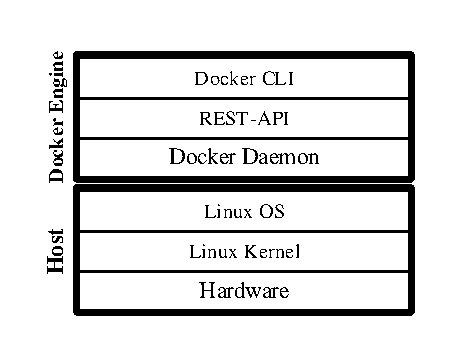
\includegraphics[scale=0.8]{images/docker-engine.pdf}
	\caption{Docker Engine architecture}
	\label{fig:docker-engine}
\end{figure} 

The Docker Engine was initially designed for LXC exclusively but has been ported to Windows. Docker Images and Containers created for Windows OS are not supported on a Linux OS and visa versa. The Docker Images and Containers for a Windows OS differ from those for a Linux OS, but the principles of Docker Images and Docker Containers are the same.

\mysubsubsection{Docker Daemon}
\label{sec:docker-daemon}
The Docker Daemon represents the background process, which creates, runs and manages the Docker Containers on the Docker Host, similar to a VM Hypervisor. The Docker Daemon strongly depends on the kernel of the host OS, therefore incompatibilities could cause the Docker Daemon to fail functioning. The communication with the Docker Daemon is performed via a REST-API, because the Docker Engine is designed as a server client architecture. \\

\mysubsubsection{REST-API}
\label{sec:docker-rest-api}
The REST-API can be exposed via a Unix socket or a network interface, depending on the configuration of the Docker Daemon. If the REST-API is exposed via a network interface, then it is recommended to secure the connection with client certificate authentication. If the Docker Engine and the Docker Client are located on the same host, then commonly the REST-API is exposed via a Unix socket and does not need any special security. \\

\mysubsubsection{Docker Command Line interface}
\label{sec:docker-cli}
The Docker Engine provides a Docker Command Line Interface (CLI) for interacting with the Docker Daemon via a Linux shell. The Docker CLI itself communicates with the Docker Daemon via the exposed REST-API. This is the most common way to interact with a Docker Daemon. The Docker CLI provides commands for creating Docker Images and Containers and for provisioning the Docker Containers on the Docker Host. \\

\mysubsubsection{Docker Images}
\label{sec:docker-images}
Docker Images are defined via Dockerfiles, which contain instructions how to build the Docker Image. A Docker Image consists of layers, where each layer represents a state of the file system, produced by a Dockerfile instruction. Each layer is immutable and any change on the file system produces a new layer. Docker Images are hierarchical and can inherit from another Docker Image, which is then called base image. Docker Images support only single inheritance and the base image is defined via the \mentionedtext{FROM} instruction as the first instruction in the Dockerfile. Docker Image names have the structure \mentionedtext{[namespace]/[name]:[version]} e.g. \mentionedtext{library/openjdk:8-alpine}. \\

\mysubsubsection{Docker Containers}
\label{sec:docker-containers}
A Docker Container is an instance of a Docker Image, where a new layer is appended, which contains all changes made on the file system by the running process within the Docker Container. When the Docker Container is deleted, then the appended layer gets deleted as well and all made changes on the file system are lost. A Docker Container keeps running as long as the contained foreground process is running. Without a foreground process the Docker Container stops immediately after it was started. The process running in the Docker Container is isolated from other processes, as well is the file system, the process has access to. \\

\subsection{Docker Architecture}
\label{sec:docker-architecture}
The Figure \vref{fig:docker-architecture} illustrates the Docker architecture, which is a client server architecture. The design as a client server architecture is the reason why the communication to the Docker Daemon is performed via the provided REST-API. The Docker Client communicates with the Docker Daemon via the Docker CLI, where the Docker Client can be located on a remote host or on the Docker Host. The Docker Host hosts the Docker Engine, which exposes the REST-API the Docker Client connects to. The Docker Engine managed the Docker Images and Containers located on the Docker Host. The Docker Engine can pull Docker Images from a remote Docker Registry, if a registry has been registered.

\begin{figure}[htbp]
	\centering
	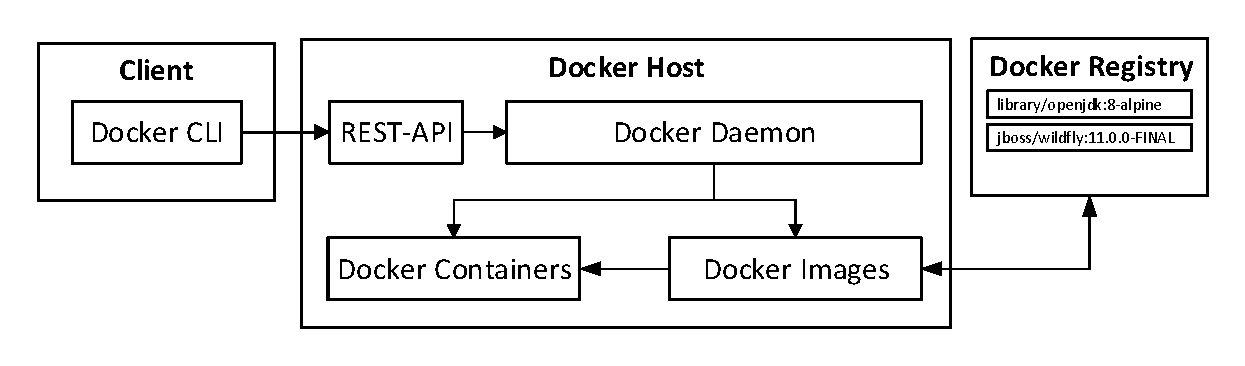
\includegraphics[scale=0.9]{images/docker-architecture.pdf}
	\caption{Docker Architecture}
	\label{fig:docker-architecture}
\end{figure} 

\subsection{Docker Machine}
\label{sec:docker-machine}
Docker Machine is a tool for managing local or remote Docker Hosts \cite{DockerMachine2018}. With Docker Machine an administrator can manage multiple Docker Hosts from a main server, without the need to connect to the Docker Host via secure shell (SSH). The Docker Machine CLI provides all commands necessary for managing Docker Hosts. Docker Engine provisions Docker Containers on a Docker Host and Docker Machine provisions Docker Hosts, in particular Docker Engines installed on docker Hosts. With Docker Machines a network of Docker Hosts can be managed, which is used by cloud platforms such as Openshift to manage Docker Engines on the nodes within the Openshift cluster.  

\section{Virtualization vs. Containerization}
\label{sec:docker-virtualization-vs-containerization}
Before LXC the industry made heavy use of operating system (OS) virtualization to isolate their environments and applications. A VM is managed by a Hypervisor, which is software, which can create, run and manage VMs. The VM provides resources such as network and storage for the application, which is managed by the virtualized OS. Nevertheless, an VM represents a full blown OS, which itself has a resource need which adds to the resource needs of the hosted application. LXC on the other hand are a kernel technology, which provides resources such as network and storage to the application as well, but without the need of virtualized OS.

\subsection{Virtual Machines}
\label{sec:docker-virtual-machines}
A Virtual Machine is an instance of a Virtual Machine Image (VMI), which is managed by a Virtual Machine Monitor (VMM), which is also referred to as the Hypervisor. The actual difference between a VMM and a Hypervisor is where the software is installed on. If the software is directly installed on the Hardware, then the software is called a Hypervisor, if its installed on the Host OS then its called a VMM. The VM abstracts  an Guest OS from the Host OS, in particular from the underlying hardware. A VM contained Guest OS is not bound to the underlying hardware, because the Hypervisor performs a kernel emulation, which allows to virtualize any Guest OS on any hardware, if the hypervisor supports it. The following Figure \ref{fig:docker-virtualization-architecture} illustrates the architecture of a virtualization system.

\begin{figure}[htbp]
	\centering
	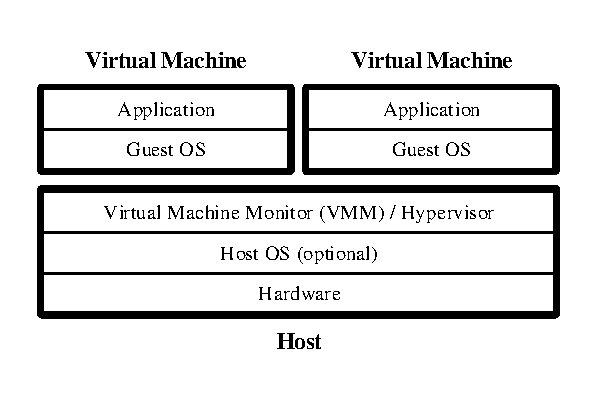
\includegraphics[scale=0.8]{images/docker-virtualization-architecture.pdf}
	\caption{Architecture of virtualized applications}
	\label{fig:docker-virtualization-architecture}
\end{figure} 

Glauber Costa's started the abstract of his talk at the LinuxCon 2012 with the humorous note \mentionedtext{"I once heard that Hypervisors are the living proof of operating system's incompetence"}. With this note he expressed that OS weren't able to provide proper isolation for applications and therefore the industry started to provide an OS instance for each application \cite{LxConCosta2012}. This has been overcome with the upcoming of LXC, which provide the proper isolation of applications on the same OS, which made the need for an OS instance for each application obsolete.

\subsection{Linux Container}
\label{sec:docker-linux-container}
The upcoming of LXC has eliminated the shortcoming to not be able to isolate applications properly of the Linux OS, which lead to using OS virtualization to isolate applications. LXC provide the feature of isolating applications running on the same OS, without the need of a kernel and hardware emulation as it is done with OS virtualization. As illustrated in Figure \ref{fig:docker-container-architecture}, the application process, binaries and libraries are bundled into the container and are isolated from other containers. Each container gets a portion o the global resources such as CPU cycles and memory assigned and cannot consume more as it has been assigned to. Without LXC it is possible that one process takes over the system resources and other processes get into state of starvation, which lead to need of OS virtualization. 

\begin{figure}[htbp]
	\centering
	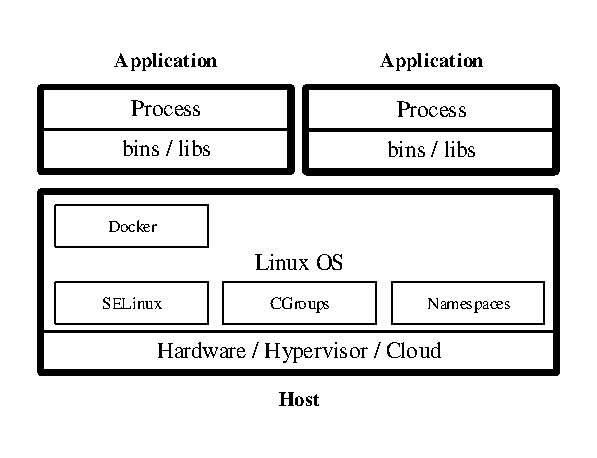
\includegraphics[scale=0.8]{images/docker-containerized-architecture.pdf}
	\caption{Architecture of containerized applications}
	\label{fig:docker-container-architecture}
\end{figure} 

The two most important kernel features underlying LXC are \mentionedtext{Cgroups} and \mentionedtext{Namespaces}. These two kernel features provide the resource control and isolation needed for application isolation and prevention of process starvation.

\mysubsubsection{Cgroups}
Cgroups stands for control groups and Cgroups provide the ability to aggregate processes, their child processes and threads within theses processes to groups managed in a tree structure. Each group gets a portion of the global resources such as CPU time, memory, I/O and network assigned, where its guaranteed that a group and its managed processes cannot consume more resources as the group has been assigned to. Each application hosted in a container is assigned to a group, where an application cannot steal resources from another application anymore, because the resource assignments of an group managed by Cgroups prevents this from happening \cite{KernelCGroupsV12018, KernelCGroupV22015, IntelLXCHyperVisor2014}. \\

\mysubsubsection{Namepsaces}
Cgroups manage how many resources can be used by processes in a group and namespaces manage the view of the system to processes. A container is managed in a namespace and therefore it has a limited view of the system such as networks and Process IDs (PIDs), depending on the configuration of the namespace the container is part of. Namespaces are a fundamental concept of LXC, and namespaces provide the isolation of a container \cite{LinuxNamespaces2018, IntelLXCHyperVisor2014}. \\

Docker has made the usage of LXC simple, but it is very hard to maintain a large set of Docker Containers (>100) via the Docker CLI, or to implement and maintain a cluster of Docker Hosts with Docker Machine. To much would have to be scripted manually, which would fast become very hard to maintain. Additionally, Docker does not provide any workflow for deployment and scaling of Docker Containers, and also does not ensure that a desired state of the containers is met. For a local development or a small set of containers the Docker CLI, Docker Compose and Docker Machine are suitable, but when it comes to large dynamic infrastructures with a large set of Docker Containers to maintain, then container orchestration platforms like Kubernetes, which is discussed in Chapter \vref{cha:caas}, will have to be used \cite{DockerSwarm2018, CNCFKubernetes2018}. 
 


%\include{chapters/figures}
%\include{chapters/mathematics}
%\section{Literature index}
\label{sec:literature-index}
The following sites are representative for the literature which will be used as theoretical base and state of the art for the thesis.

\cite{PicozziHepburnConnor2017}
\cite{Morris2017}
\cite{Newman2015}
\cite{HohpeWoolf2003}
\cite{DockerDoc}
\cite{MartinFowlerBlog}
\cite{OpenshiftDoc}
\cite{redHatJBossFuse}

\bibliography{references}
\bibliographystyle{amsalpha}

%\include{chapters/printing}
%\include{chapters/closing}

%%%----------------------------------------------------------
\appendix                                         % appendix 
%%%----------------------------------------------------------

%\chapter{Technical Details}
\label{app:TechnicalDetails}



	% technical supplements
%\chapter{CD-ROM/DVD Contents}
\label{app:cdrom}


	% contents of the CD-ROM/DVD
%\chapter{Questionnaire}
\label{app:Questionnaire}





	% chronological list of changes
%\chapter{\latex Source Code}
\label{app:SourceCode}

	% source text of this document

%%%----------------------------------------------------------
\MakeBibliography                        				% references
\listoffigures                                          % all figures
\listoflistings                                         % all listings
%%%----------------------------------------------------------
%%% special page for checking print size --------------------
%\chapter*{Check Final Print Size}

\begin{center}
{\Large --- Check final print size! ---}

\bigskip

\calibrationbox{100}{50} % width/height of box in mm

\bigskip

{\Large --- Remove this page after printing! ---}

\end{center}



%%%----------------------------------------------------------
\end{document}
%%%----------------------------------------------------------